%  English version of main.tex (reviewer observation 4). Same content, tables and numbers as the
%  Spanish manuscript of 18/11/2026; figures with English labels (*_en.png, a15_figuras_en.py).
%  Compile: latexmk -pdf main_en.tex
%=================================================================
\documentclass[sensors,article,submit,pdftex,moreauthors]{Definitions/mdpi}

\firstpage{1}
\makeatletter
\setcounter{page}{\@firstpage}
\makeatother
\pubvolume{1}
\issuenum{1}
\articlenumber{0}
\pubyear{2026}
\copyrightyear{2026}
\datereceived{ }
\daterevised{ }
\dateaccepted{ }
\datepublished{ }

%=================================================================
\usetikzlibrary{positioning,arrows.meta}

%=================================================================
\Title{Lightweight YOLO Detectors for Tomato Pests and Diseases under High Solar Radiation: Leakage-Free Evaluation, Robustness to Overexposure, and Offline Deployment}

\Author{Fray Benjamin Kana Chullo $^{1,}$*, Hiram Jeremy Ccoto Cruz $^{1}$ and Angel Rosendo Condori Coaquira $^{1}$}

\AuthorNames{Fray Benjamin Kana Chullo, Hiram Jeremy Ccoto Cruz and Angel Rosendo Condori Coaquira}

\address{%
$^{1}$ \quad Professional School of Systems Engineering, Faculty of Engineering and Architecture, Universidad Peruana Unión, Juliaca, Peru}

\corres{Correspondence: fray.kana@upeu.edu.pe}

\abstract{High solar radiation in arid regions overexposes field photographs and can hide white pests such as whitefly or powdery mildew. We measured this effect on lightweight YOLO detectors (YOLOv8n, YOLO11n and YOLOv10n) trained on 1966 tomato images from the Majes Valley (Peru), using a capture-group split, three seeds and labels corrected after an audit. On the test set, the four-class mAP@0.5 was $26.5 \pm 3.8$\% (YOLOv8n: $29.8$\%). At midday, saturated pixels quadrupled. When the same photos were synthetically overexposed, mAP@0.5 fell by 32\% with one exposure step and whitefly lost two thirds of its AP; underexposure had no effect. Photometric augmentation raised retention at two steps (42\% vs.\ 29\%; better in 9 of 9 runs) at the cost of 2.4 points under normal light; CLAHE equalization did not help. No strategy recovered whitefly beyond 1.5 steps, so mitigation must include image capture (shading or exposure). Enlarging the dataset improved the new sessions, not the original one. A mid-range phone processed each photo in about 0.6~s offline. Data, code and models are public.}

\keyword{solar radiation; overexposure; photometric augmentation; whitefly; powdery mildew; \emph{Tuta absoluta}; data leakage; group split; small object detection; edge inference}

\begin{document}

%=================================================================
\section{Introduction}

In the Majes Valley (Arequipa, Peru), tomato is grown under high solar irradiance and on plots where technical assistance does not always arrive in time. Deep-learning object detectors can locate several lesions in a single photo~\cite{Fuentes2017}, and lightweight versions of the YOLO family can run on a phone~\cite{Zhong2024,Wang2025}. However, results obtained with laboratory images do not transfer to the field~\cite{Mohanty2016,Jelali2024}.

Two problems are less studied. The first is evaluation: when each plant is photographed several times and the photos are split at random, near-identical images end up in both training and test, and the metrics are inflated~\cite{Kapoor2023}. In tomato disease detection, data augmentation applied before splitting the dataset inflated mAP50 by up to 66 percentage points~\cite{Gerz2025}. The second is illumination: high radiation causes overexposure and specular reflections that can hide the white mycelium of powdery mildew or the body of the whitefly (\emph{Bemisia tabaci}), an object that is already small for one-stage detectors~\cite{Zhang2024Jute,Zhao2025}.

The \textbf{objective} of this work was to evaluate, without data leakage, lightweight YOLO detectors for four tomato pests and diseases (late blight, powdery mildew, whitefly and tomato leafminer) in a region of high solar radiation, to measure how much overexposure degrades them, to test two ways of mitigating it, and to verify their operation on an offline phone. Five research questions were posed:
\begin{itemize}[leftmargin=*,labelsep=4.9mm]
\item \textbf{Q1.} What data leakage exists when splitting by image, and how much remains after splitting by capture group?
\item \textbf{Q2.} Does the detector improve when the dataset is enlarged with new field sessions, evaluated on the same images and labels?
\item \textbf{Q3.} How much does photo exposure change across time bands, and how much does overexposure degrade the detector, per class?
\item \textbf{Q4.} Do photometric augmentation or CLAHE preprocessing reduce this degradation, and at what cost under normal light?
\item \textbf{Q5.} How useful is the detector for diagnosis (including the error of declaring an infested plant healthy), and is its performance preserved on the phone?
\end{itemize}

%=================================================================
\section{Related Work}

Table~\ref{tab:relacionados} summarizes closely related work. Accuracies above 98\% are obtained with laboratory images on uniform backgrounds~\cite{Mohanty2016,Debnath2023}; with field images, values drop and depend on object size and on how the data are split~\cite{Jelali2024}. \citet{Shehu2025} detected \emph{Tuta absoluta} damage with YOLOv8 on 326 field photos from three farms in Nigeria (mAP up to 0.737), without edge deployment. \citet{Zhao2025} counted whiteflies with YOLOv11 and sliced inference (SAHI) on 5124 images of 50~MP (mAP50 of 91.6\%), with inference on a server. \citet{Debnath2023} brought a tomato disease classifier to an Android application, trained on 10\,000 images from a public repository. None of these works measures how solar overexposure degrades the detector, nor combines it with a capture-group leakage audit and on-phone performance measurement.

\begin{table}[H]
\caption{Related work (values as reported by their authors).\label{tab:relacionados}}
\begin{adjustwidth}{-\extralength}{0cm}
\begin{tabularx}{\fulllength}{lXXXl}
\toprule
\textbf{Work} & \textbf{Data} & \textbf{Model} & \textbf{Result} & \textbf{Deployment}\\
\midrule
\citet{Debnath2023} & 10\,000 repository images, 10 classes (classification) & EfficientNetV2B2 & 98.96\% test accuracy & Android app\\
\citet{Shehu2025} & 326 field images, \emph{Tuta absoluta} & YOLOv8 & mAP up to 0.737 & Laptop\\
\citet{Zhao2025} & 5124 field images, whitefly (5 crops) & YOLOv11s + SAHI & mAP50 = 91.6\% & Server\\
This work & 1966 field images, 4 classes, 3 sessions, high radiation & YOLOv8n, YOLO11n, YOLOv10n & mAP@0.5 = 23--30\% depending on architecture; robustness to overexposure measured & Phone, offline\\
\bottomrule
\end{tabularx}
\end{adjustwidth}
\end{table}

%=================================================================
\section{Materials and Methods}

\subsection{Image Acquisition}

Photos were taken at the El Pedregal farm (Majes) in three sessions (3 May, 12 July and 29 July 2026) with a Samsung Galaxy A56 5G (50~MP), without flash and without handling the plants; frames were also extracted from short videos. Each image was assigned to a time band according to its file time: morning (before 11:00, 555 images), midday (11:00--13:59, 397) and afternoon (from 14:00, 1014). Midday was captured only in the 3 May session.

\subsection{Annotation}\label{sec:anotacion}

Two annotators from the team labeled the images in Roboflow. The main annotator (F.B.K.C.) has seven years of experience growing tomato in El Pedregal (Majes, Arequipa), on a farm advised by field agronomists, and recognizes these pests and diseases in daily crop management. Boxes of five classes were used: \emph{late blight} (\emph{Phytophthora infestans}), \emph{powdery mildew} (species not confirmed in the laboratory), \emph{whitefly} (\emph{B. tabaci}), \emph{tomato leafminer} (\emph{Tuta absoluta}; includes insect and mine) and \emph{healthy leaf}. The written rules were: one box per lesion, insect or mine; healthy leaf only for completely healthy leaflets; overlapping leaves with one box each; label everything recognizable in the foreground but nothing distant or blurred; and do not label objects smaller than 16~px at 640~px. Identification is based on symptoms visible in the field. There was no laboratory confirmation and no validation by an independent plant pathologist. Inter-annotator agreement is measured with a blind protocol (Section~\ref{sec:acuerdo}).

After the label audit (Section~\ref{sec:auditoria}), the 319 flagged images were reviewed manually. Missing late blight lesions were added (2698 $\rightarrow$ 2933 boxes, with changes in 158 images), and the healthy-leaf class was removed, because it was only partially labeled and is not a pest. Images without pests are kept as background images. This final version (v6) has four classes and 4648 boxes (Table~\ref{tab:dataset}).

\begin{table}[H]
\caption{Boxes per class and subset in the final version (v6). v5 additionally had 3356 healthy-leaf boxes and 2698 late blight boxes.\label{tab:dataset}}
\begin{tabularx}{\textwidth}{lCCCC}
\toprule
\textbf{Class} & \textbf{Training} & \textbf{Validation} & \textbf{Test} & \textbf{Total}\\
\midrule
Late blight & 1914 & 689 & 330 & 2933\\
Powdery mildew & 594 & 209 & 89 & 892\\
Tomato leafminer & 374 & 70 & 29 & 473\\
Whitefly & 253 & 63 & 34 & 350\\
\midrule
Images without pests & 308 & 77 & 33 & 418\\
\textbf{Images} & \textbf{1405} & \textbf{381} & \textbf{180} & \textbf{1966}\\
\bottomrule
\end{tabularx}
\end{table}

\subsection{Leakage-Free Split}

Photos were taken in bursts around each plant. A \emph{capture group} was defined as the set of photos in a folder taken less than 30~s apart, and each video as one group; the physical identity of the plants was not recorded. The 288 groups were assigned whole (70/20/10 by number of images within each time-band folder). In addition, a video recorded less than 30~s from a burst was merged with it: this moved 66 images (3.4\%) to the subset of their group. The training code checks both rules and stops if it finds a split group. As a time-independent check, all pairs of images from different subsets were compared with a perceptual hash (63-bit pHash).

\subsection{Models, Training and Environment}

YOLOv8n, YOLO11n and YOLOv10n~\cite{Jocher2023,Jocher2024,Wang2024v10}, pretrained on COCO, were compared with seeds 0, 1 and 2 and $640\times640$ inputs (Table~\ref{tab:entorno}). The model is selected by validation mAP@0.5:0.95, never by test results. Four versions of the dataset are described: v1 (1028 May images, split by image), v4 (1021 May images with revised labels and split by group), v5 (all 1966 images from the three sessions, five classes) and v6 (the same images and split as v5, with corrected labels and four classes).

\begin{table}[H]
\caption{Environment and hyperparameters.\label{tab:entorno}}
\begin{tabularx}{\textwidth}{lXX}
\toprule
& \textbf{v4} & \textbf{v5 and v6}\\
\midrule
Hardware & Tesla T4 GPU (Google Colab) & RTX 5070 Ti GPU, 16 GB\\
Software & Ultralytics 8.4.82 & Ultralytics 8.4.82, PyTorch 2.12, CUDA 13.2\\
Epochs / patience & 150 / 30 & 200 / 50\\
Batch & 16 & 32\\
Other & default augmentation & default augmentation, cosine learning rate, mixed precision, no mosaic in the last 15 epochs\\
\midrule
Conversion & \multicolumn{2}{p{0.72\textwidth}}{ONNX (opset 17) $\rightarrow$ onnx2tf 1.26.3 (TensorFlow 2.18.1) $\rightarrow$ TFLite float16}\\
Phone & \multicolumn{2}{p{0.72\textwidth}}{Samsung Galaxy A56 (Exynos 1580), tflite\_flutter 0.11.0, CPU with 4 threads, no delegate}\\
\bottomrule
\end{tabularx}
\end{table}

\subsection{Evaluation}

\textbf{Test subsets.} To compare v4 and v5 on the same images and the same ground truth, all evaluations use the v5 labels and three subsets of the test set: \emph{fixed test} (97 images from the v4 test set that remain in test, all from 3 May), \emph{new images} (83 images: 29 from 12 July, 51 from 29 July and 3 from 3 May) and \emph{full test} (180). Of v4, only the selected model was kept (YOLO11n, seed 1).

\textbf{Detection metrics.} Ultralytics mAP@0.5 and mAP@0.5:0.95, with the five classes and without the healthy leaf. Uncertainty was estimated with a bootstrap clustered by capture group (1000 replicates), and the v4--v5 difference with a paired bootstrap over the same images.

\textbf{Image-level metrics.} With the application rules (confidence 0.30, IoU 0.45, class-agnostic NMS): sensitivity and specificity per pest or disease (presence in the image) and the \emph{false-healthy rate}, that is, the proportion of images with some pest or disease in which the model detects none. Also the main-class accuracy (highest-confidence detection vs.\ the most frequent class in the labels), with two baselines (always answering the majority class or always healthy), Wilson intervals and McNemar's test to compare v4 and v5.

\textbf{Exposure.} Per image: percentage of saturated pixels (any channel $\geq 250$), mean brightness, contrast and a specular indicator (V $\geq 230$ and S $\leq 40$). On the test set, accuracy was compared across saturation terciles, and a logistic regression of accuracy was fitted with session and model as controls and errors clustered by capture group.

\textbf{Overexposure stress test.} Each test image was synthetically overexposed: it was converted from sRGB to linear values, multiplied by $2^{\mathrm{EV}}$, clipped at 1 and converted back to sRGB, with EV $\in \{-1, 0, +0.5, +1, +1.5, +2\}$ exposure steps. Since the only difference between versions of a photo is the exposure, the drop of the detector can be attributed to it. With +1 EV, the median share of saturated pixels in test goes from 1\% to 20\%. We report \emph{retention}: mAP@0.5 under overexposure divided by the mAP@0.5 of the same run without it.

\textbf{Mitigation.} With v6, three experiments were trained, each with the three architectures and three seeds (27 runs):
\begin{itemize}[leftmargin=*,labelsep=4.9mm]
\item \emph{baseline}: default augmentation (brightness variation of $\pm 40\%$);
\item \emph{photometric augmentation}: brightness variation of $\pm 70\%$ and one overexposed copy of each training image, with EV uniform between +0.5 and +1.5 and the same method as the stress test, in training only;
\item \emph{CLAHE}: contrast-limited adaptive histogram equalization on luminance (clip limit 2.0, $8\times8$ grid), applied to all images, including those of the stress test.
\end{itemize}
Each experiment was compared with the baseline using pairs of architecture and seed and the Wilcoxon test.

\textbf{Excess-light warning.} The application shows a ``too much light'' warning when, in the photo sampled every 6~pixels, the mean luminance exceeds 200 or more than 15\% of the pixels exceed 240. The warning was validated on the 180 photos of each stress-test level with the installed model (v6) and the application rules. An image with pests was considered correct if any detected class matched the labeled ones. A \emph{light-induced failure} was defined as an image--level pair that is correct with the original exposure and fails when overexposed.

\textbf{Inter-annotator agreement and external validation.}\label{sec:acuerdo} A stratified sample of 100 v6 images was drawn: 20 with tomato leafminer, 20 with whitefly, 20 with powdery mildew, 25 with late blight and 15 without pests, from the three sessions and with a single image per capture group (258 reference boxes). The two annotators relabel it independently, without seeing the existing labels or each other's, using the written rules and four classes. Image-level agreement is summarized with Cohen's kappa on the presence of each class, and box-level agreement with the F1 of boxes matched per class (IoU $\geq 0.5$ and $\geq 0.3$). Each annotator is also compared with the v6 labels. In addition, an external agronomist classifies 50 of those images (10 per stratum) by marking the classes present, and their kappa with the v6 labels is computed.

\textbf{Phone.} An automated test passed 192 images through the same application code and measured the time from the JPEG bytes to the final boxes and the agreement with the server (same main class; boxes with the same class and IoU $\geq 0.5$).

\subsection{System}

The application (Flutter) analyzes the photo on the server (FastAPI) when a connection is available and on the phone itself with TFLite when it is not; results are stored in SQLite and synchronized later (Figure~\ref{fig:arq}). Both sides correct the EXIF orientation and use a 640~px letterbox with the same thresholds; they differ in the resizing interpolation (OpenCV on the server and the Dart \texttt{image} library on the phone).

\begin{figure}[H]
\centering
\resizebox{0.95\linewidth}{!}{%
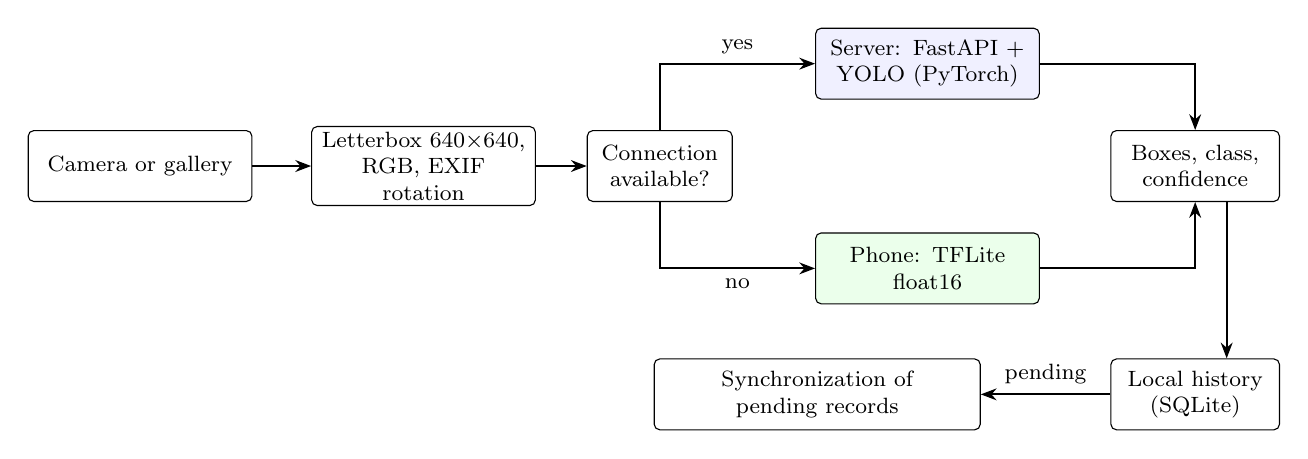
\begin{tikzpicture}[
  font=\footnotesize,
  box/.style={draw, rounded corners=2pt, align=center, minimum height=9mm, text width=27mm, inner sep=2pt, fill=white},
  arr/.style={-{Stealth[length=2mm]}, thick}
]
\node[box] (cam) at (0,0) {Camera or gallery};
\node[box] (pre) at (3.6,0) {Letterbox 640$\times$640,\\RGB, EXIF rotation};
\node[box, text width=17mm] (route) at (6.6,0) {Connection\\available?};
\node[box, fill=blue!6] (srv) at (10,1.3) {Server: FastAPI +\\YOLO (PyTorch)};
\node[box, fill=green!8] (tfl) at (10,-1.3) {Phone: TFLite\\float16};
\node[box, text width=20mm] (res) at (13.4,0) {Boxes, class,\\confidence};
\node[box, text width=20mm] (db) at (13.4,-2.9) {Local history\\(SQLite)};
\node[box, text width=40mm] (sync) at (8.6,-2.9) {Synchronization of\\pending records};
\draw[arr] (cam) -- (pre);
\draw[arr] (pre) -- (route);
\draw[arr] (route.north) |- node[pos=0.75, above]{yes} (srv.west);
\draw[arr] (route.south) |- node[pos=0.75, below]{no} (tfl.west);
\draw[arr] (srv.east) -| (res.north);
\draw[arr] (tfl.east) -| (res.south);
\draw[arr] (res.south) ++(4mm,0) -- ([xshift=4mm]db.north);
\draw[arr] (db) -- node[above]{pending} (sync);
\end{tikzpicture}}
\caption{Architecture with inference on the server or on the phone.\label{fig:arq}}
\end{figure}

\subsection{Availability and Reproducibility}

The dataset is available on Roboflow Universe under a CC~BY~4.0 license~\cite{Dataset2026}: version~1 corresponds to v4, version~2 to v5 and version~3 to v6. The research repository contains the training code (which verifies the split and applies the 66 moves), the image lists of each test subset, the metrics of each run, the models and the scripts of this analysis (Table~\ref{tab:repro}). Since v5 and v6 were trained with \texttt{deterministic=False}, a new run may differ slightly.

\begin{table}[H]
\caption{Public resources.\label{tab:repro}}
\begin{adjustwidth}{-\extralength}{0cm}
\begin{tabularx}{\fulllength}{lX}
\toprule
\textbf{Resource} & \textbf{Link}\\
\midrule
Dataset & \url{https://universe.roboflow.com/fray-hxtls/plagas-tomate-majes-v2}\\
Code, results and models & \url{https://github.com/fraykanachullo/trabajoinvestigacionTomate}\\
Server (FastAPI) & \url{https://github.com/fraykanachullo/backentTomate}\\
Mobile application (Flutter) & \url{https://github.com/fraykanachullo/frontendTomate}\\
\bottomrule
\end{tabularx}
\end{adjustwidth}
\end{table}

%=================================================================
\section{Results}

\subsection{Q1: Data Leakage}

In v1, split by image, 65 of 189 capture groups had photos in more than one subset, and 82 of the 103 test images had a photo of the same group in training or validation. Its validation mAP@0.5 was 30.2--30.6\% in three YOLOv8n configurations with one seed. v4, already split by group, obtained 27.7--30.4\% in validation and 21.5--24.2\% in test. Since the split, the labels and the image format changed at the same time between v1 and v4, this difference does not isolate the effect of leakage; a controlled experiment with the same labels remains as future work.

In the final split, the comparison of the 856\,785 pairs of images from different subsets found no near-identical pair: the minimum pHash distance was 12, and the only pair at that distance corresponds to different scenes. For reference, two photos from the same burst are at a median distance of 30. This method rules out duplicate photos, but not the same plant photographed in two separate bursts.

\subsection{Q2: Effect of Enlarging the Dataset}

Table~\ref{tab:v4v5} and Figure~\ref{fig:modelos} compare the v4 model with the v5 models on the same images. On the \emph{fixed test} (May), v5 did not improve: without the healthy leaf it obtained an mAP@0.5 of 17.6--21.3\% vs.\ 19.2\% for v4, and all paired differences had a 95\% CI including zero (for example, with five classes, YOLOv8n seed 2 minus v4: $-2.5$ points, CI $-7.5$ to $+2.3$). On the \emph{new images} (July), which v4 never saw, v5 went from 25.8\% to 32.1--44.4\%. The 95\% CI of a model's mAP@0.5 on the fixed test spans about $\pm$6--8 points, so differences between architectures (0.5 to 3.7 points on average) fall within the uncertainty.

\begin{table}[H]
\caption{mAP@0.5 (\%) with the v5 labels on the three test subsets; v5 as mean $\pm$ SD of 3 seeds. ``4 classes'' excludes the healthy leaf.\label{tab:v4v5}}
\begin{adjustwidth}{-\extralength}{0cm}
\begin{tabularx}{\fulllength}{lCCCCCC}
\toprule
& \multicolumn{2}{c}{\textbf{Fixed test (97)}} & \multicolumn{2}{c}{\textbf{New images (83)}} & \multicolumn{2}{c}{\textbf{Full test (180)}}\\
\textbf{Model} & \textbf{5 classes} & \textbf{4 classes} & \textbf{5 classes} & \textbf{4 classes} & \textbf{5 classes} & \textbf{4 classes}\\
\midrule
v4: YOLO11n, s1 & 26.6 & 19.2 & 32.1 & 25.8 & 27.9 & 21.9\\
v5: YOLOv8n & $25.1 \pm 0.6$ & $17.6 \pm 2.9$ & $46.8 \pm 5.4$ & $39.5 \pm 7.4$ & $33.6 \pm 2.5$ & $25.8 \pm 3.4$\\
v5: YOLO11n & $24.6 \pm 0.8$ & $18.4 \pm 1.0$ & $41.7 \pm 8.7$ & $32.1 \pm 11.7$ & $32.2 \pm 3.9$ & $24.0 \pm 4.9$\\
v5: YOLOv10n & $28.3 \pm 0.9$ & $21.3 \pm 0.9$ & $49.6 \pm 5.3$ & $44.4 \pm 6.4$ & $36.3 \pm 1.1$ & $29.8 \pm 1.3$\\
\bottomrule
\end{tabularx}
\end{adjustwidth}
\end{table}

\begin{figure}[H]
\centering
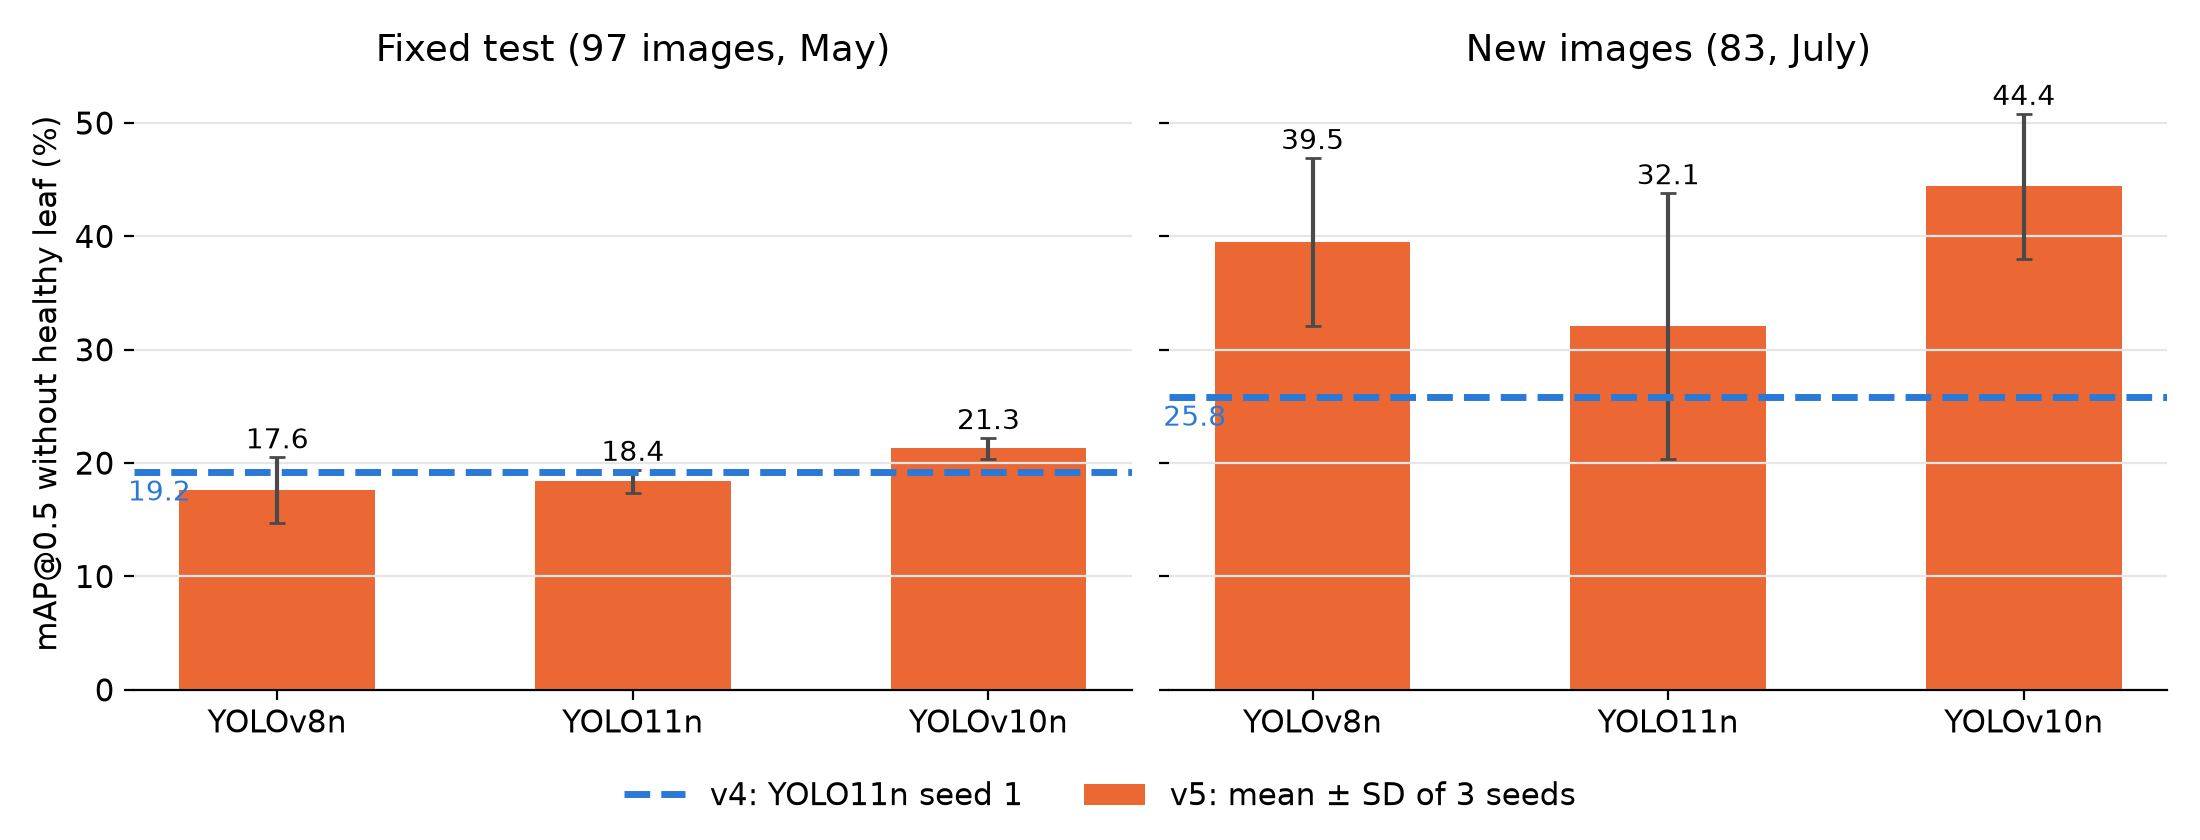
\includegraphics[width=0.92\textwidth]{fig_v4_v5_modelos_en.png}
\caption{mAP@0.5 without the healthy leaf on the same images and labels: v5 matches v4 on the May photos and surpasses it on the July photos.\label{fig:modelos}}
\end{figure}

Per class (Figure~\ref{fig:clases}), on the full test v5 obtained the highest AP@0.5 for tomato leafminer (38--62\% depending on the architecture) and whitefly (24--33\%); late blight stayed at 20--26\% and powdery mildew at 5--8\%. The new images contain no powdery mildew box (Section~\ref{sec:auditoria}). The best validation point was reached between epochs 24 and 79; afterwards, the validation classification loss increased.

\begin{figure}[H]
\centering
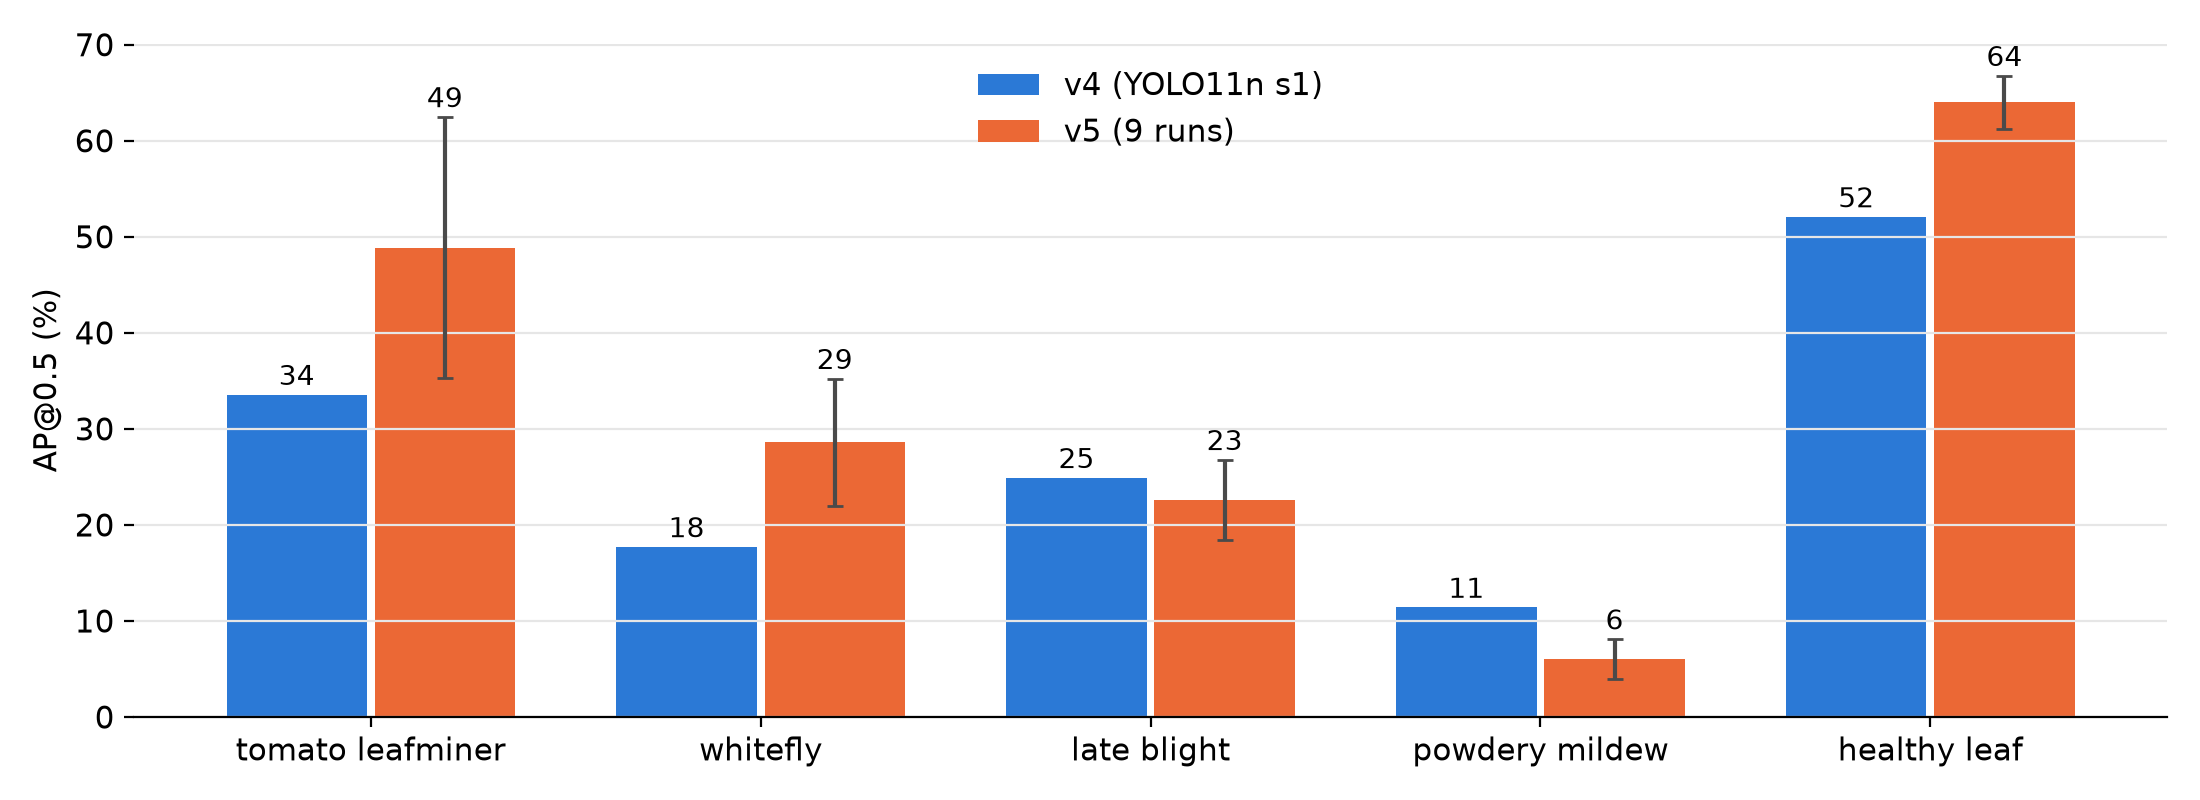
\includegraphics[width=0.92\textwidth]{fig_v4_v5_clases_en.png}
\caption{AP@0.5 per class on the full test (180 images; 29 tomato leafminer boxes, 34 whitefly boxes, 89 powdery mildew boxes).\label{fig:clases}}
\end{figure}

\subsection{Q3: Solar Exposure}

At midday, the median share of saturated pixels was 3.6\% vs.\ 0.8\% in the morning and 1.0\% in the afternoon, and contrast was higher (58.8 vs.\ 48.7 and 51.0; Figure~\ref{fig:exposicion}). On the test set, the main-class accuracy (9 v5 models) fell from 67\% in the lowest saturation tercile to 57\% and 55\% in the middle and high terciles, with overlapping intervals. With session and model as controls, the odds ratio per standard deviation of saturation was 0.82 (95\% CI: 0.65--1.04; $p = 0.11$); brightness (OR = 1.00) and the specular indicator (OR = 0.98) were not associated with accuracy. The high saturation tercile comes almost entirely (55 of 60 images) from the May session, so with the real photos exposure cannot be separated from session.

\begin{figure}[H]
\centering
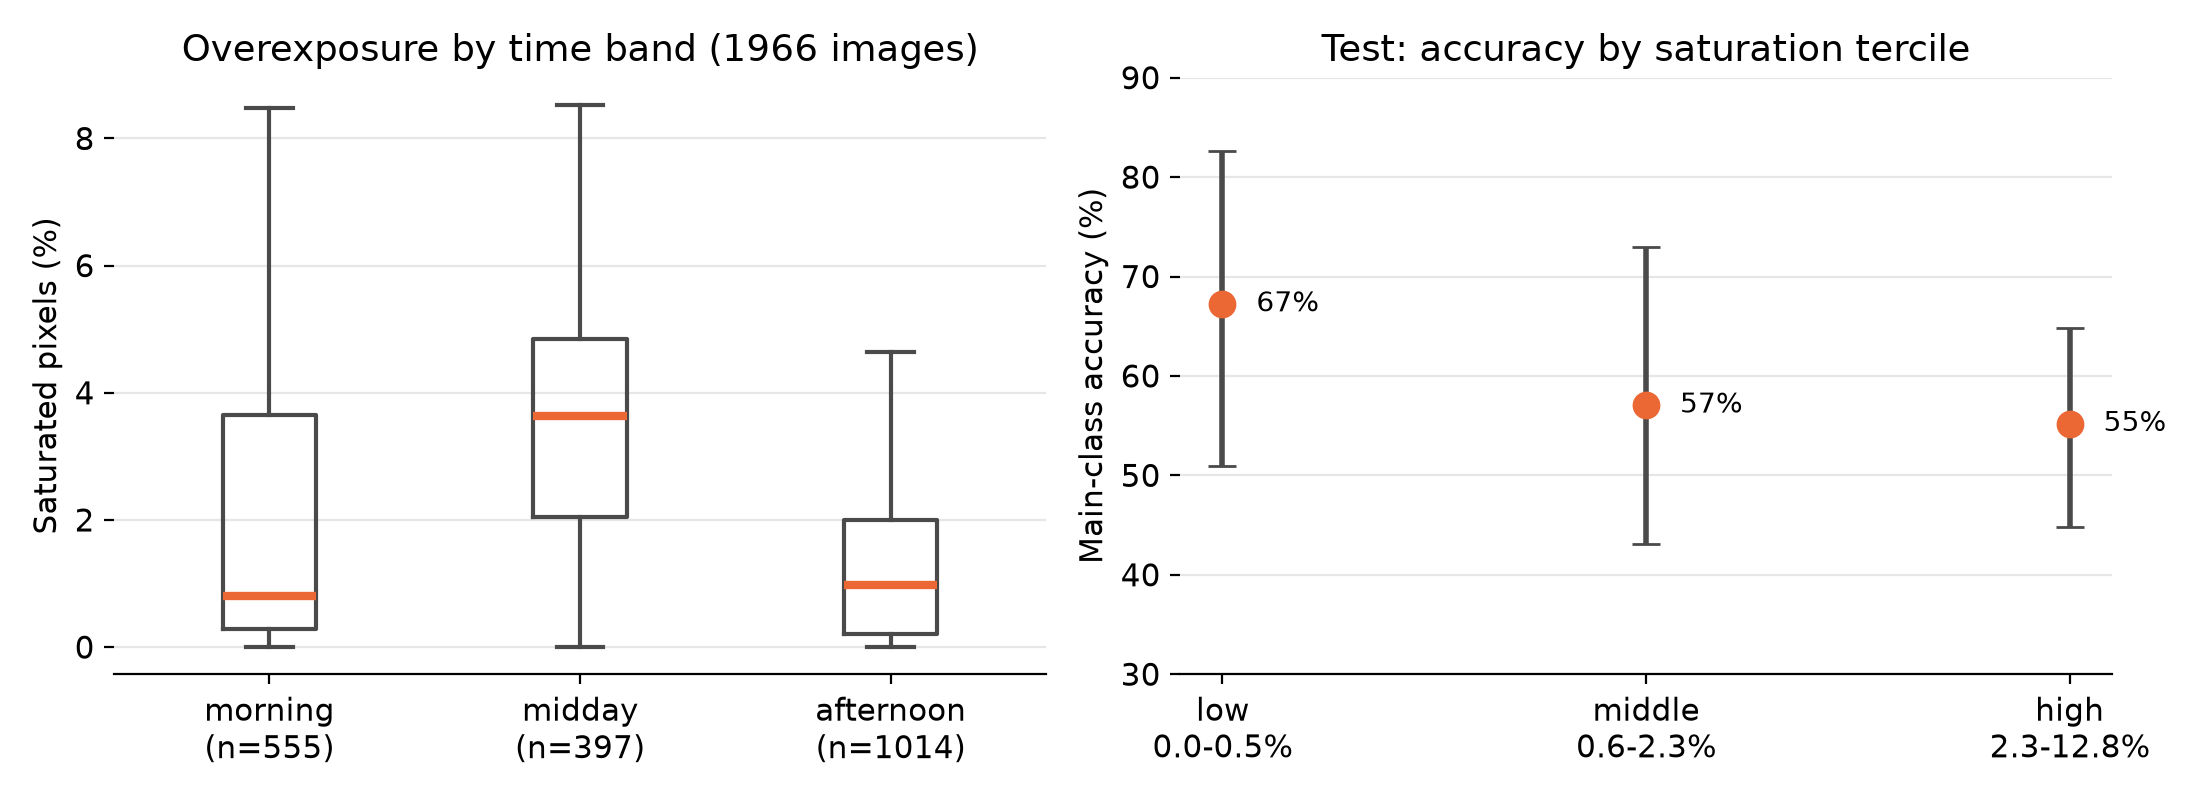
\includegraphics[width=0.92\textwidth]{fig_exposicion_en.png}
\caption{Left: saturated pixels by time band. Right: main-class accuracy by saturation tercile on the test set, with 95\% CI from a clustered bootstrap.\label{fig:exposicion}}
\end{figure}

The stress test does separate the effect, because it compares the same photo with different exposure (Figure~\ref{fig:estres}, baseline curves). With the v6 baseline models, mAP@0.5 went from 26.3\% with the original exposure to 23.0\% with +0.5 EV, 17.9\% with +1 EV and 7.5\% with +2 EV. The effect is gradual and occurs only with excess light: with $-1$ EV, mAP@0.5 did not change (25.6\%). The white classes are the most sensitive. Whitefly dropped from 30.6\% to 22.2\% with +0.5 EV and to 9.8\% with +1 EV, and powdery mildew from 6.4\% to 2.7\% with +1 EV. Tomato leafminer, with dark lesions, held up to +1 EV (from 47.6\% to 42.3\%). The false-healthy rate rose from 44\% to 51\% with +1 EV and to 65\% with +2 EV. The nine five-class v5 models showed the same curve. The real photos lie at the start of the curve: the midday median saturation (3.6\%) lies between 0 and +0.5 EV, and the maximum (12.8\%) between +0.5 and +1 EV.

\subsection{Q4: Mitigation of Overexposure}

With the corrected labels and four classes (v6), the baseline model obtained a test mAP@0.5 of $26.5 \pm 3.8\%$. By architecture, YOLOv8n obtained $29.8 \pm 3.2$, YOLO11n $26.4 \pm 1.0$ and YOLOv10n $23.4 \pm 3.9$, vs.\ 25.8, 24.0 and 29.8 for v5 without the healthy leaf. Per class, tomato leafminer obtained 47.7\%, whitefly 31.5\%, late blight 20.6\% and powdery mildew 6.4\%. On average, correcting the labels and removing the healthy leaf did not change the overall level; the test labels also changed, so the comparison with v5 is approximate.

Table~\ref{tab:mitigacion} and Figure~\ref{fig:estres} compare the strategies. Photometric augmentation consistently reduced the loss from overexposure: with +2 EV, all nine runs retained more than their baseline pair (42\% vs.\ 29\%; $+13.3$ points, $p = 0.004$). With +1.5 EV, seven of nine runs retained more than the baseline ($p = 0.074$). With +1 EV and above, its absolute mAP@0.5 was the highest. This augmentation had a cost under normal light. It decreased in validation ($-3.4$ points, $p = 0.008$) and on the fixed test ($-2.4$, $p = 0.039$), and declared more infested images healthy ($+8.5$ points, $p = 0.16$). The robustness gain was concentrated in YOLOv8n and YOLO11n: their retention at +1 EV was 80\%, vs.\ 70\% and 67\% for the baseline. In YOLOv10n it was 69\% vs.\ 67\%. CLAHE did not significantly improve any metric. No strategy rescued whitefly at +1.5 EV or more (AP@0.5 of 3\% in all three cases).

The application's ``too much light'' warning did not appear in any of the 180 real test photos. It appeared in 8\% of the images at +0.5 EV, in 61\% at +1 EV and in 98--99\% at +1.5 and +2 EV. Among the 280 combinations of image and overexposed level that the model got right with the original exposure, 110 became failures. The warning detected 79\% of these light-induced failures (specificity 44\%). With the warning, the failure rate was 48\%, vs.\ 24\% without it. Lowering the threshold of pixels $> 240$ to 5\% would raise detection to 92\%, but the warning would appear on 3\% of normal photos. With 25\%, Youden's index improves little ($J = 0.28$ vs.\ 0.23).

\begin{table}[H]
\caption{Mitigation experiments with v6 (four classes): mean $\pm$ SD of 9 runs (3 architectures $\times$ 3 seeds). Retention: mAP@0.5 under overexposure divided by the original mAP@0.5 of the same run.\label{tab:mitigacion}}
\begin{adjustwidth}{-\extralength}{0cm}
\begin{tabularx}{\fulllength}{lCCCCCCC}
\toprule
& \multicolumn{3}{c}{\textbf{Normal light}} & \multicolumn{4}{c}{\textbf{Stress test}}\\
\cmidrule(lr){2-4}\cmidrule(lr){5-8}
\textbf{Experiment} & \textbf{Test mAP@0.5} & \textbf{Fixed-test mAP@0.5} & \textbf{False healthy} & \textbf{mAP@0.5, +1 EV} & \textbf{Retention +1 EV} & \textbf{Retention +2 EV} & \textbf{Whitefly AP, +1 EV}\\
\midrule
Baseline & $26.5 \pm 3.8$ & $20.2 \pm 2.8$ & $44.4 \pm 8.6$ & $17.9 \pm 3.1$ & $68 \pm 9$ & $29 \pm 5$ & $9.8 \pm 4.3$\\
Photometric & $25.1 \pm 4.1$ & $17.8 \pm 2.4$ & $52.9 \pm 16.8$ & $19.1 \pm 5.0$ & $76 \pm 11$ & $42 \pm 10$ & $14.5 \pm 9.3$\\
CLAHE & $24.6 \pm 3.7$ & $18.0 \pm 3.5$ & $45.4 \pm 12.5$ & $17.2 \pm 3.7$ & $69 \pm 7$ & $31 \pm 8$ & $11.2 \pm 7.3$\\
\bottomrule
\end{tabularx}
\end{adjustwidth}
\end{table}

\begin{figure}[H]
\begin{adjustwidth}{-\extralength}{0cm}
\centering
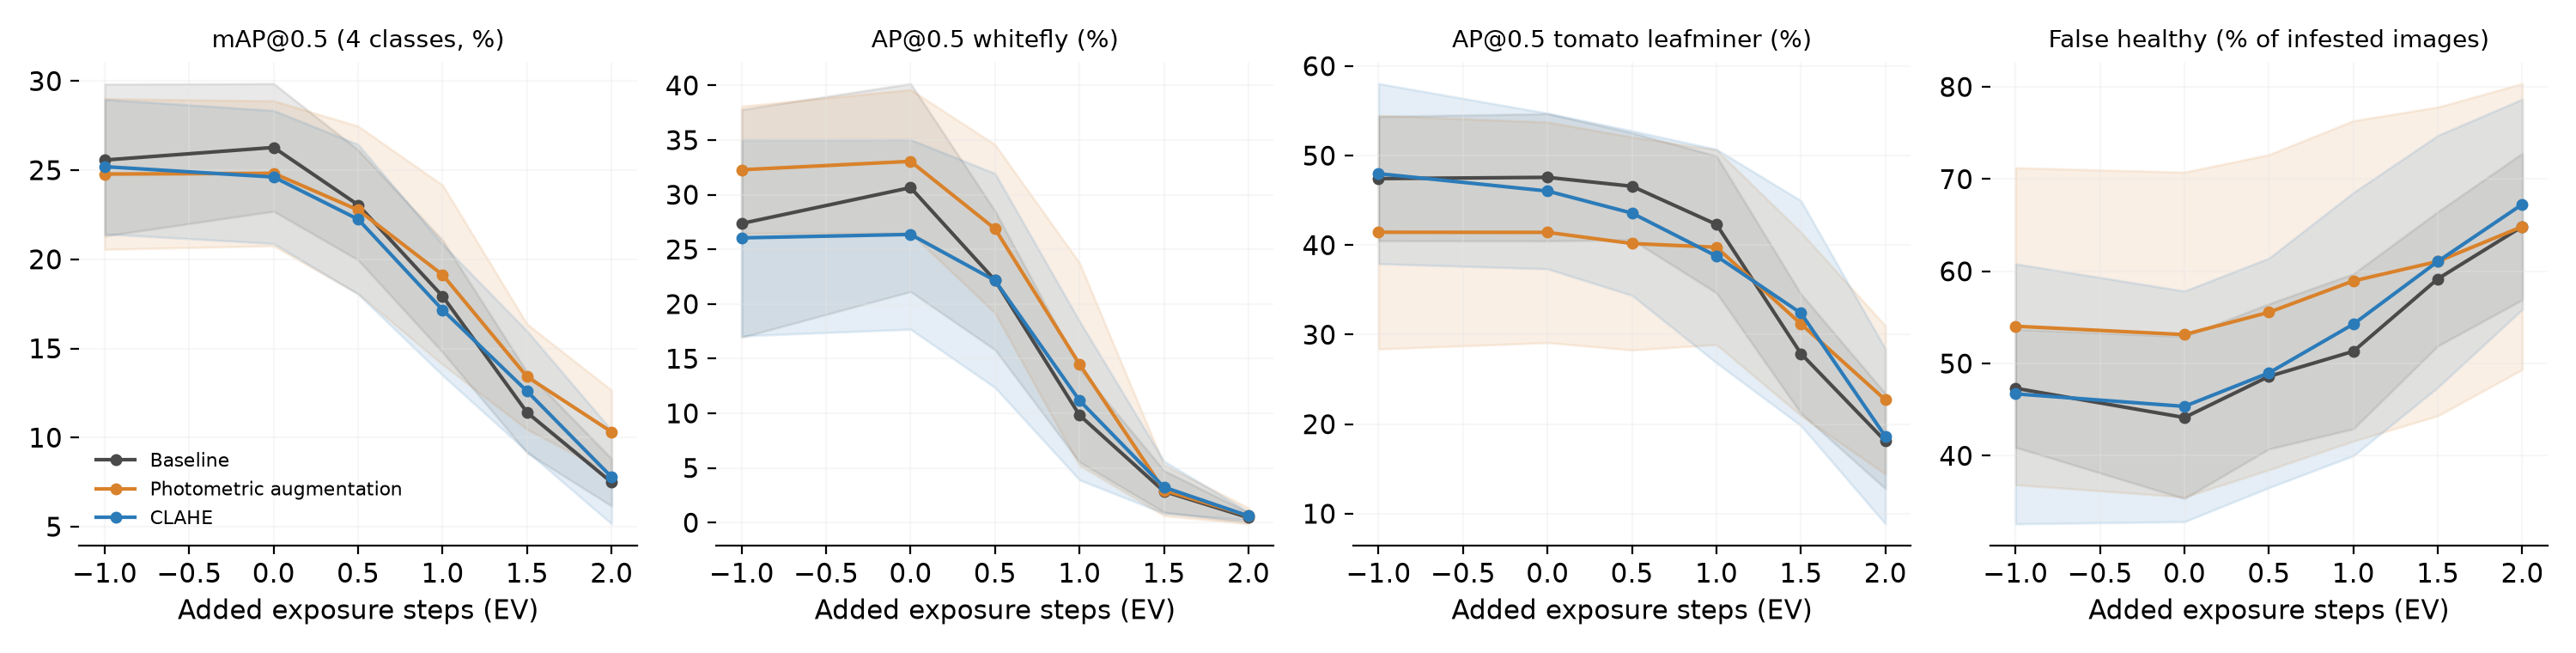
\includegraphics[width=\linewidth]{fig_estres_v6_en.png}
\end{adjustwidth}
\caption{Stress test: the 180 test photos synthetically overexposed (added exposure steps). Mean of 9 runs per experiment; the band is $\pm 1$ SD across runs.\label{fig:estres}}
\end{figure}

\subsection{Q5: Diagnostic Usefulness and Performance on the Phone}

Table~\ref{tab:imagen} shows the image-level metrics. The installed v5 model (YOLOv8n seed 2) detected no pest in 28\% of the infested images (false healthy; 40 of 144), vs.\ 22\% for v4 (32 of 144); among the nine v5 models this value ranged from 27\% to 52\%. On the fixed test, always answering ``late blight'' gets the main class right in 60.8\% of the images, a value similar to that of the models; on the full test, the models (51--67\%) do outperform the baselines (41.1\% and 26.7\%). On the fixed test, three of the nine v5 models were significantly less accurate than v4 (McNemar, $p < 0.01$); the installed model did not differ from it ($p = 0.29$). With the v6 baseline (four classes, same rules), the false-healthy rate was $44.4 \pm 8.6\%$ (33--60\% across runs; 38\% for the YOLOv8n selected by validation): correcting the labels did not reduce this error.

\begin{table}[H]
\caption{Image-level metrics on the full test (180 images; 144 with some pest or disease), with the application rules. In brackets, 95\% Wilson CI.\label{tab:imagen}}
\begin{adjustwidth}{-\extralength}{0cm}
\begin{tabularx}{\fulllength}{lCCCCCC}
\toprule
\textbf{Model} & \textbf{Main-class accuracy} & \textbf{False healthy} & \textbf{Sens. late blight} & \textbf{Sens. whitefly} & \textbf{Sens. powdery mildew} & \textbf{Sens. leafminer}\\
\midrule
v4: YOLO11n, s1 & 66.1\% [58.9--72.6] & 22.2\% [16.2--29.7] & 71\% & 37\% & 59\% & 55\%\\
v5: YOLOv8n, s2 & 63.9\% [56.6--70.5] & 27.8\% [21.1--35.6] & 64\% & 37\% & 41\% & 52\%\\
v5: range of 9 models & 51--67\% & 27--52\% & 40--73\% & 13--43\% & 6--59\% & 21--59\%\\
Baseline ``always late blight'' & 41.1\% & 0\% & 100\% & 0\% & 0\% & 0\%\\
\bottomrule
\end{tabularx}
\end{adjustwidth}
\end{table}

On the phone, the v4 model processed a photo in $501 \pm 120$~ms and assigned the same main class as the server in 83.9\% of 192 images (95\% CI: 78.0--88.4); 80.4\% of the server boxes were reproduced. With the same input, the TFLite and ONNX versions agree on the main detection in 96 of 96 images (maximum confidence difference of 0.004 for v4 and 0.014 for v5), so the disagreement with the server comes mainly from the different interpolation used when downscaling the photo, which changes the winning detection when confidences are close to the 0.30 threshold. The v6 model (YOLOv8n baseline, four classes) replaced v5 on the server and in the application. Converted to TFLite float16 (6.1~MB), it agrees with the ONNX version on the main detection in 96 of 96 images, with a maximum confidence difference of 0.004. On the phone, with the same 192 images, the v6 model processed a photo in $574 \pm 186$~ms (median 596~ms) in a second run. The first run, right after installing the application, gave $756 \pm 497$~ms (median 673~ms), and the detections were identical in both. Most of the time is spent decoding and downscaling the photo: the median was 271~ms for images under 1~MP and 678~ms for the 50~MP photos. The v6 model assigned the same main class as the server in 82.8\% of the images (95\% CI: 76.8--87.5), similar to v4. It reproduced 77.0\% of the server boxes, and 82.0\% of its own boxes matched those of the server. Figure~\ref{fig:app} shows the application; the screenshots were taken by pointing the phone at field photos shown on a monitor.

\begin{figure}[H]
\centering
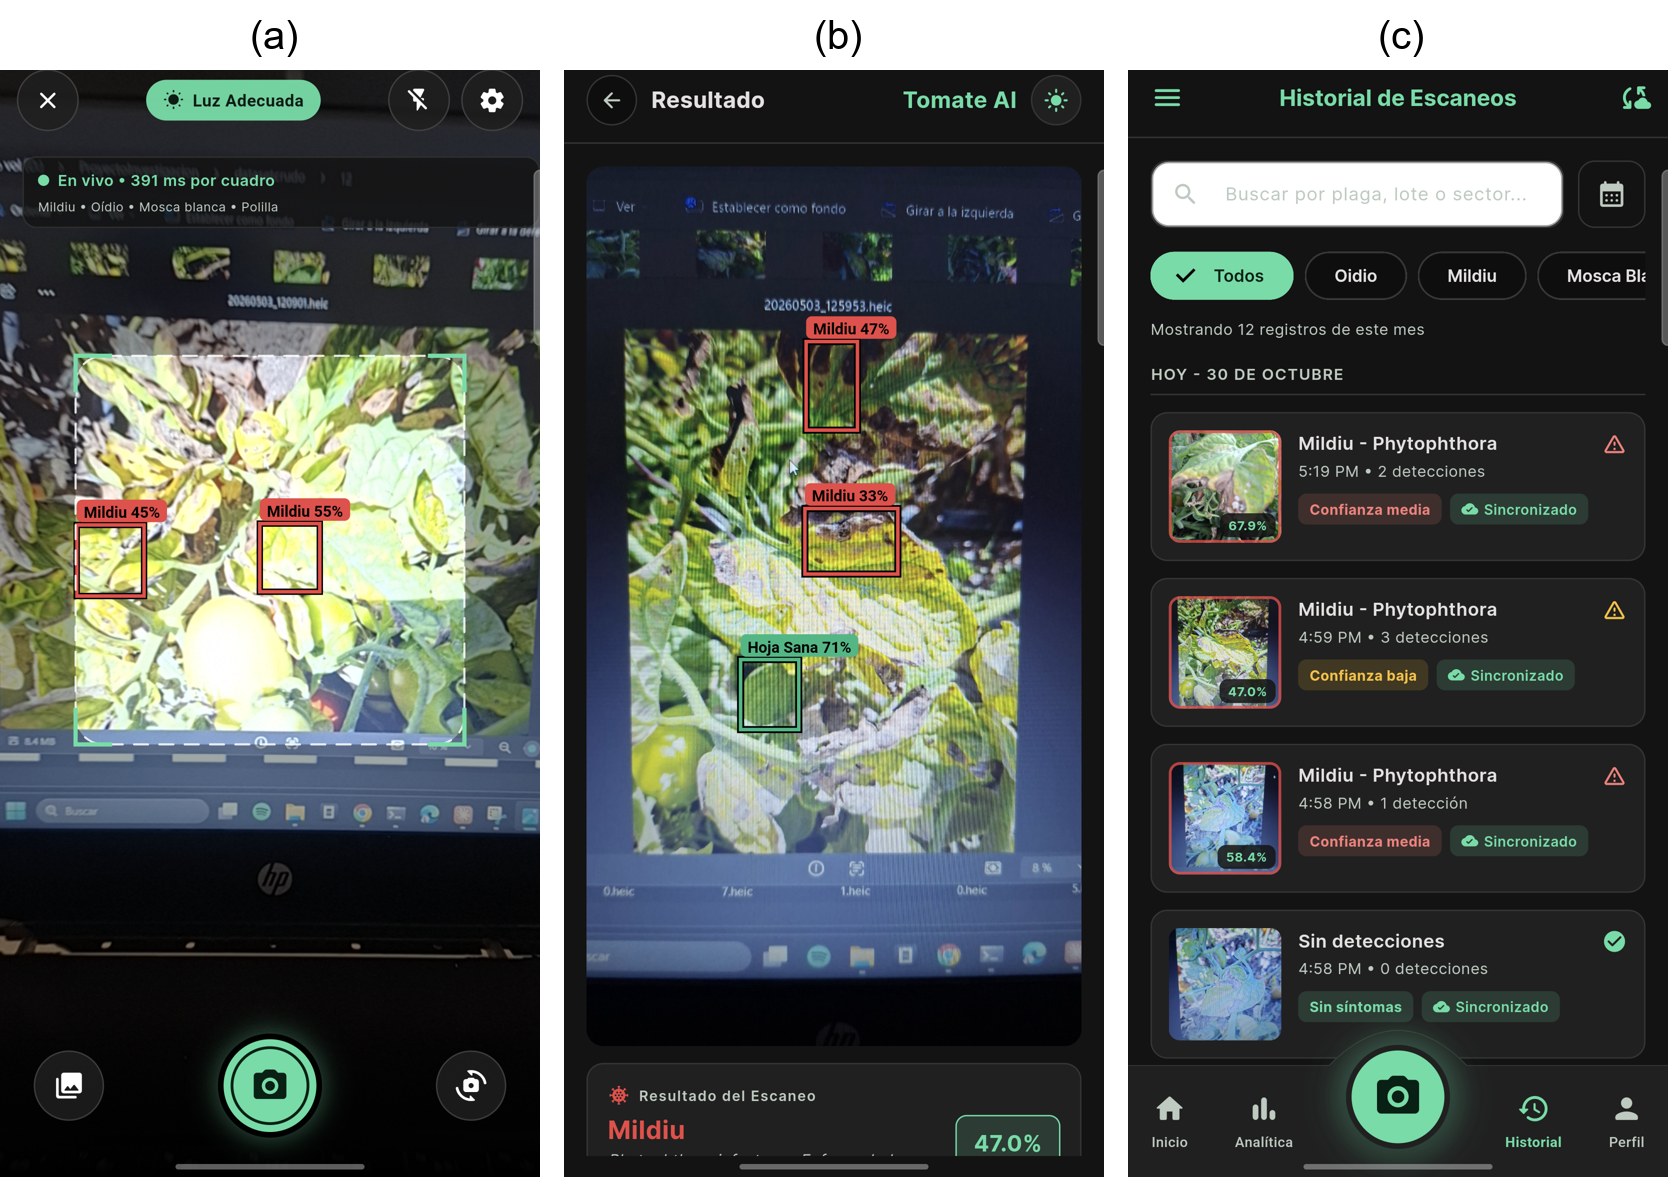
\includegraphics[width=0.9\textwidth]{fig_app_capturas.png}
\caption{Application on the Samsung Galaxy A56 (v4 model; Spanish interface), with field photos shown on a monitor: (a) live mode; (b) result of a photo; (c) synchronized history.\label{fig:app}}
\end{figure}

\subsection{Label Audit}\label{sec:auditoria}

To find labeling errors, the nine v5 models were used as reviewers on validation and test (561 images), together with a structural review of all 1966 images (Figure~\ref{fig:auditoria}). Four problems were found: (i) powdery mildew is labeled almost only in May: 869 boxes in the v4 images vs.\ 20 in the 944 new images, and 118 of its 295 validation and test boxes are detected by no model; (ii) the late blight criterion changes by session: the median box area is 0.20\% of the image on 12 July and 1.49\% on 29 July (a spot vs.\ the affected leaf); (iii) the healthy leaf is only partially labeled: in 212 cases the nine models agree on a healthy leaf without a box; and (iv) 87\% of the whitefly boxes (302 of 349) measure less than 16~px at 640~px. Only two boxes would have the wrong class and there are no duplicate boxes: the problem is not the assigned class, but how much and how each object is enclosed. In v6 the missing late blight was completed, which partially corrects problem (ii), and the healthy leaf was removed, which resolves (iii) (Section~\ref{sec:anotacion}); (i) and (iv) require new captures.

\begin{figure}[H]
\centering
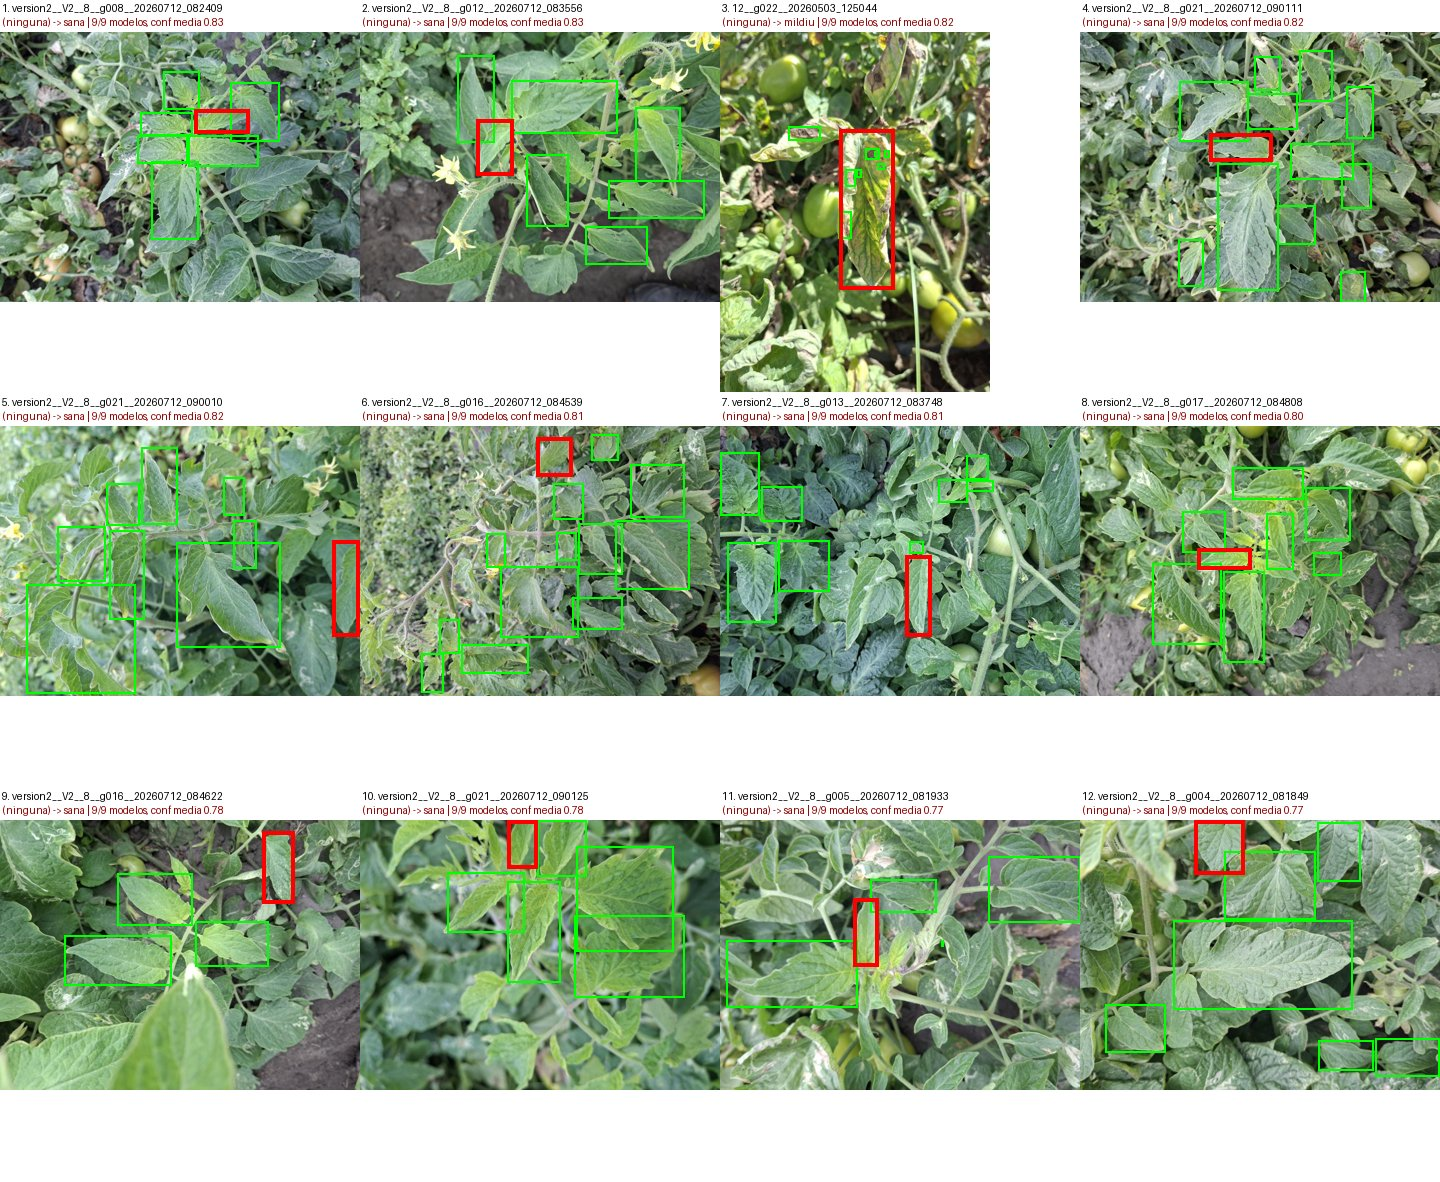
\includegraphics[width=0.95\textwidth]{fig_auditoria.jpg}
\caption{Audit examples: in green, the labeled boxes; in red, objects that the nine models detect without a box (healthy leaves and a late blight lesion).\label{fig:auditoria}}
\end{figure}

%=================================================================
\section{Discussion}

\textbf{Enlarging the dataset improved generalization to new sessions, not performance under the original conditions.} With the same images and labels, v5 did not outperform v4 on the May photos, but it did on the July photos. The practical lesson is that capturing on different dates and plants contributes more than adding photos under the same conditions. Since some hyperparameters also changed between v4 and v5 (Table~\ref{tab:entorno}) and only one v4 model was kept, this comparison should be confirmed by retraining v4 with the v5 configuration.

\textbf{The architectures are equivalent at this scale.} Among the three lightweight detectors evaluated at 640~px, differences between architectures were smaller than the variation between seeds and than the CI of the test set. YOLOv8n is kept because it wins on validation, is the fastest to train and the application already processes its output format; choosing YOLOv10n because it wins on the v5 test would bias the estimate~\cite{Kapoor2023}. In v6, YOLOv8n was the best on validation and on test, and YOLOv10n the worst. The conclusion is limited to nano models, which are the ones that fit on the phone.

\textbf{The classes that improved were those that received more new examples, but this effect cannot be separated from label size and quality.} Tomato leafminer and whitefly, with more new boxes, improved on the July images; powdery mildew did not, and the audit shows it was hardly labeled in July. Whitefly lies below the size that a detector resolves at 640~px; \citet{Zhao2025} managed to count it with 50~MP images and sliced inference, an alternative to increasing the input resolution. The four-class mAP@0.5 of 23--30\% is low compared with the works in Table~\ref{tab:relacionados}, which use laboratory images, a single object type or splits that do not control leakage~\cite{Gerz2025}.

\textbf{Overexposure degrades the detector gradually, and above all on white objects.} On the real photos, accuracy tended to decrease with saturation without reaching significance, because exposure was confounded with session. The stress test removed this confounding and showed a dose--response relationship. One exposure step, which leaves 20\% of the pixels saturated, removed one third of the mAP@0.5 and two thirds of the whitefly AP. This supports the initial hypothesis: the white body of the insect and the powdery mildew mycelium are confused with burned-out areas, whereas the dark lesions of the tomato leafminer hold up. Current midday photos are already in the range where whitefly starts to be lost.

\textbf{Photometric augmentation buys robustness at the expense of accuracy under normal light; CLAHE does not address this problem.} Training with overexposed copies taught the model to tolerate burned-out photos: retention at +2 EV improved in every run. But with normal photos the model performs somewhat worse and declares more infested plants healthy. The choice depends on the real light of use. With the current saturation distribution, around 0 to +0.5 EV, the baseline model is preferable. If the field test shows many photos above +1 EV, the photometric model is preferable. CLAHE redistributes contrast, but it does not recover saturated pixels, whose information is already lost.

\textbf{Beyond 1.5 steps, mitigation must happen when the photo is taken.} No training or preprocessing strategy recovered whitefly once the insect was saturated. The practical mitigation is to shade the leaf with one's body or an umbrella, correct the phone's exposure or warn the user. The application's ``too much light'' warning serves this purpose. It does not appear on normal photos, it triggers from about +1 EV, and when it appears the model fails twice as often. Its thresholds were therefore kept, and the message now tells the user to shade the leaf. Its specificity is low (44\%) because many overexposed photos are still classified correctly. In addition, it covers the +0.5 EV range poorly, where whitefly already starts to be lost. The paired sun-and-shade field test must confirm whether shading recovers accuracy.

\textbf{Correcting the labels did not raise the ceiling; the data set it.} After adding the missing late blight and removing the healthy leaf, the average mAP@0.5 did not change. Powdery mildew still has almost no examples in July, with an AP of 6\%, and whitefly is still tiny. Improving requires more examples of these classes with a single criterion, not more training adjustments.

\textbf{The costliest error for the farmer is the false healthy.} Between a quarter and almost half of the infested cases are declared healthy, depending on the model. Therefore, before using the application to decide on a treatment, it should show the confidence and ask the user to check again when it detects nothing on a plant with symptoms.

\subsection{Limitations}\label{sec:limitaciones}

(i) The classes were identified by visible symptoms, without laboratory confirmation; the field experience of the main annotator does not replace an independent validation; the audit found inconsistent criteria; and the results of the inter-annotator agreement and the external validation (Section~\ref{sec:acuerdo}) will be added once completed; (ii) the capture group is defined by time and not by plant identity, so leakage between bursts of the same plant cannot be ruled out; (iii) the test set has 180 images and few tomato leafminer (29) and whitefly (34) boxes; (iv) midday was captured in only one session, and synthetic overexposure does not reproduce specular reflections or hard shadows, so a paired field test is still needed (the same leaves in sun and shade, with measured irradiance); (v) only one v4 model was kept and hyperparameters changed between v4 and v5, and the controlled leakage experiment (random split vs.\ group split with the same labels) was prepared but not run; (vi) with three seeds, the SD between runs is of the same order as several differences between experiments; (vii) phone latency was measured with images served from a PC and not with the camera, the resizing interpolation still differs between server and phone, the light warning was validated with synthetic overexposure and not with field photos, and the application was not tested in the field.

%=================================================================
\section{Conclusions}

A dataset of 1966 tomato field images from a region of high solar radiation was built and published. It is split by capture group, has no duplicate images between subsets, and its labels were corrected after an audit. Lightweight YOLO detectors reached an mAP@0.5 of 23--30\% on four pests and diseases, with differences between architectures smaller than the uncertainty. Enlarging the dataset with new sessions improved performance on those sessions, but not under the original conditions.

Overexposure degrades the detector gradually and, above all, on whitefly and powdery mildew. Photometric augmentation reduces this loss at the cost of some accuracy under normal light, and CLAHE does not reduce it. Beyond 1.5 exposure steps, only better image capture can prevent the loss. The system works offline on a mid-range phone.

Future work is to:
\begin{itemize}[leftmargin=*,labelsep=4.9mm]
\item carry out the paired field test (the same leaves in three time bands, with a lux meter and shade at midday) to validate the stress curve and the application warning;
\item validate the classes with a specialist and measure inter-annotator agreement;
\item run the controlled leakage experiment;
\item test a higher resolution or sliced inference for whitefly;
\item match the resizing between server and phone and test the application in the field.
\end{itemize}

%=================================================================
\vspace{6pt}

\authorcontributions{Conceptualization, F.B.K.C. and H.J.C.C.; methodology, F.B.K.C. and H.J.C.C.; software, F.B.K.C.; investigation and data curation, F.B.K.C. and H.J.C.C.; writing---original draft preparation, F.B.K.C.; writing---review and editing, H.J.C.C. and A.R.C.C.; supervision, A.R.C.C. All authors have read and agreed to the published version of the manuscript.}

\funding{This research received no external funding.}

\institutionalreview{Not applicable: the study did not involve humans or animals.}

\informedconsent{Not applicable.}

\dataavailability{The dataset is available on Roboflow Universe under a CC~BY~4.0 license (\url{https://universe.roboflow.com/fray-hxtls/plagas-tomate-majes-v2}). The code, the lists of each test subset, the metrics and the models are available at \url{https://github.com/fraykanachullo/trabajoinvestigacionTomate}; the server and application code, in the repositories of Table~\ref{tab:repro}.}

\acknowledgments{We thank the owners of the El Pedregal farm (Majes) for access to the field. An artificial intelligence assistant (Claude, Anthropic) was used in the preparation of the manuscript and the analysis code; the authors reviewed all the content and take full responsibility for it.}

\conflictsofinterest{The authors declare no conflicts of interest.}

%=================================================================
\begin{adjustwidth}{-\extralength}{0cm}
\reftitle{References}
\begin{thebibliography}{999}

\bibitem[Fuentes et~al.(2017)]{Fuentes2017}
Fuentes, A.; Yoon, S.; Kim, S.C.; Park, D.S. A robust deep-learning-based detector for real-time tomato plant diseases and pests recognition. {\em Sensors} {\bf 2017}, {\em 17}, 2022. \url{https://doi.org/10.3390/s17092022}.

\bibitem[Zhong(2024)]{Zhong2024}
Zhong, Y. Tomato leaf disease identification based on YOLOv8. {\em Int. J. Comput. Sci. Inf. Technol.} {\bf 2024}, {\em 3}, 265--276. \url{https://doi.org/10.62051/ijcsit.v3n2.30}.

\bibitem[Wang and Liu(2025)]{Wang2025}
Wang, X.; Liu, J. TomatoGuard-YOLO: A novel efficient tomato disease detection method. {\em Front. Plant Sci.} {\bf 2025}, {\em 15}, 1499278. \url{https://doi.org/10.3389/fpls.2024.1499278}.

\bibitem[Mohanty et~al.(2016)]{Mohanty2016}
Mohanty, S.P.; Hughes, D.P.; Salath\'e, M. Using deep learning for image-based plant disease detection. {\em Front. Plant Sci.} {\bf 2016}, {\em 7}, 1419. \url{https://doi.org/10.3389/fpls.2016.01419}.

\bibitem[Jelali(2024)]{Jelali2024}
Jelali, M. Deep learning networks-based tomato disease and pest detection: A first review of research studies using real field datasets. {\em Front. Plant Sci.} {\bf 2024}, {\em 15}, 1493322. \url{https://doi.org/10.3389/fpls.2024.1493322}.

\bibitem[Kapoor and Narayanan(2023)]{Kapoor2023}
Kapoor, S.; Narayanan, A. Leakage and the reproducibility crisis in machine-learning-based science. {\em Patterns} {\bf 2023}, {\em 4}, 100804. \url{https://doi.org/10.1016/j.patter.2023.100804}.

\bibitem[Gerz and Jelali(2025)]{Gerz2025}
Gerz, F.; Jelali, M. Towards reliable data augmentation in machine learning: Practices to prevent data leakage [data and code]. Mendeley Data, version 1, 2025. \url{https://doi.org/10.17632/f9k79z29rp.1}.

\bibitem[Zhang et~al.(2024)]{Zhang2024Jute}
Zhang, S.; Wang, H.; Zhang, C.; Liu, Z.; Jiang, Y.; Yu, L. JutePest-YOLO: A deep learning network for jute pest identification and detection. {\em IEEE Access} {\bf 2024}, {\em 12}, 72938--72956.

\bibitem[Zhao et~al.(2025)]{Zhao2025}
Zhao, S.; Lyu, J.; Liu, S.; Feng, Z.; Ling, H.; Jiao, J.; Ni, Z.; Yang, B.; Yao, Q.; Luo, J. A counting method of whiteflies on crop leave images captured by AR glasses based on segmentation and improved YOLOv11 models. {\em Front. Plant Sci.} {\bf 2025}, {\em 16}, 1687282. \url{https://doi.org/10.3389/fpls.2025.1687282}.

\bibitem[Debnath et~al.(2023)]{Debnath2023}
Debnath, A.; Hasan, M.M.; Raihan, M.; Samrat, N.; Alsulami, M.M.; Masud, M.; Bairagi, A.K. A smartphone-based detection system for tomato leaf disease using EfficientNetV2B2 and its explainability with artificial intelligence (AI). {\em Sensors} {\bf 2023}, {\em 23}, 8685. \url{https://doi.org/10.3390/s23218685}.

\bibitem[Shehu et~al.(2025)]{Shehu2025}
Shehu, H.A.; Ackley, A.; Mark, M.; Eteng, O.E.; Sharif, M.H.; Kusetogullari, H. YOLO for early detection and management of \emph{Tuta absoluta}-induced tomato leaf diseases. {\em Front. Plant Sci.} {\bf 2025}, {\em 16}, 1524630. \url{https://doi.org/10.3389/fpls.2025.1524630}.

\bibitem[Jocher et~al.(2023)]{Jocher2023}
Jocher, G.; Chaurasia, A.; Qiu, J. Ultralytics YOLOv8, 2023. Available online: \url{https://github.com/ultralytics/ultralytics}.

\bibitem[Jocher and Qiu(2024)]{Jocher2024}
Jocher, G.; Qiu, J. Ultralytics YOLO11, 2024. Available online: \url{https://github.com/ultralytics/ultralytics}.

\bibitem[Wang et~al.(2024)]{Wang2024v10}
Wang, A.; Chen, H.; Liu, L.; Chen, K.; Lin, Z.; Han, J.; Ding, G. YOLOv10: Real-time end-to-end object detection. In {\em Advances in Neural Information Processing Systems 37 (NeurIPS 2024)}, 2024. \url{https://arxiv.org/abs/2405.14458}.

\bibitem[Kana Chullo(2026)]{Dataset2026}
Kana Chullo, F.B. plagas-tomate-majes-v2 Dataset. Roboflow Universe, 2026. License CC BY 4.0. Available online: \url{https://universe.roboflow.com/fray-hxtls/plagas-tomate-majes-v2}.

\end{thebibliography}
\end{adjustwidth}
\end{document}
